% Created 2019-05-23 Thu 00:46
% Intended LaTeX compiler: pdflatex
\documentclass[presentation]{beamer}
\usepackage[utf8]{inputenc}
\usepackage[T1]{fontenc}
\usepackage{graphicx}
\usepackage{grffile}
\usepackage{longtable}
\usepackage{wrapfig}
\usepackage{rotating}
\usepackage[normalem]{ulem}
\usepackage{amsmath}
\usepackage{textcomp}
\usepackage{amssymb}
\usepackage{capt-of}
\usepackage{hyperref}
\usepackage{awesomebox}
\usepackage{booktabs}
\usepackage{placeins}
\usepackage{siunitx}
\usepackage{minted}
\usetheme[progressbar=frametitle]{metropolis}
\usepackage{tikz}
\usepackage{tikz-3dplot}
\usetikzlibrary{intersections,calc,shapes.geometric}
\usepackage{pgfplots}
\pgfplotsset{compat=newest}
\usepackage{spot}
\newcommand{\gv}[1]{\ensuremath{\mbox{\boldmath$ #1 $}}}
\newcommand{\bv}[1]{\ensuremath{\mathbf{#1}}}
\newcommand{\norm}[1]{\left\lVert#1\right\rVert}
\newcommand{\abs}[1]{\left\lvert#1\right\rvert}
\newcommand{\bigqm}[1][1]{\text{\larger[#1]{\text{?}}}}
\newcommand{\order}[1]{\mathcal O \left( #1 \right)} % order of magnitude
\definecolor{scarlet}{rgb}{1.0, 0.13, 0.0}
\definecolor{shamrockgreen}{rgb}{0.0, 0.62, 0.38}
\definecolor{royalblue}{rgb}{0.25, 0.41, 0.88}
\definecolor{metropolisorange}{RGB}{235,129,27}
\definecolor{metropolisblue}{RGB}{35,55,59}
\usetheme{default}
\author{\emph{Tejaswin Parthasarathy}, Mattia Gazzola}
\date{\today}
\title{Elastica : Spatial discretization}
\subtitle{ME498: Comp. modeling \& optimization}
\hypersetup{
 pdfauthor={\emph{Tejaswin Parthasarathy}, Mattia Gazzola},
 pdftitle={Elastica : Spatial discretization},
 pdfkeywords={},
 pdfsubject={},
 pdfcreator={Emacs 27.0.50 (Org mode 9.2)},
 pdflang={English}}
\begin{document}

\maketitle
\tikzset{>=latex}
\section{Introduction}
\label{sec:org5589b72}
\begin{frame}[label={sec:org05b01cc}]{Integration and differentiation of functions}
More specifically numerical integration (\alert{quadrature}) and differentiation
\begin{block}{Integration}
Given \(a, b, f\) compute a numerical approximation to
\[ \int_{a}^{b} f(x) dx \]
For purposes of this course, we assume \(f\) is Riemann integrable
  \(\Rightarrow\) Integral exists and is unique
\end{block}
\begin{block}{Differentiation}
Given \(a, b, f\) compute a numerical approximation to
\[ \frac{df}{dx} \; \in \; [a,b]\]
Again we assume \(f\) is smooth enough (\(C^{r}\;\in\;[a,b]\))
\end{block}
\end{frame}
\begin{frame}[label={sec:org436f568}]{Where are these useful?}
\begin{block}{Everywhere!}
\begin{itemize}
\item We \emph{integrated} quantitites in time in the last lecture (IVPs and
timeseries analysis)
\item Anything involving spatial quantities (BVPs, including solving PDEs using
finite differences/volume/element, spectral element and so on\ldots{})
\end{itemize}
\end{block}
\end{frame}
\begin{frame}[label={sec:orga2c1b8e}]{Outline}
\begin{itemize}
\item More about quadrature, and what to look for in a quadrature rule
\item Simple (yet effective) quadrature schemes and their derivation
\item Do the same for numerical differentiation
\item Give context to these methods in our soft mechanics framework
\end{itemize}
\end{frame}
\section{Quadrature}
\label{sec:org3e827f5}
\begin{frame}[label={sec:orgf875be2}]{Interpolatory quadrature}
\begin{itemize}
\item Design a quadrature method based on interpolation of values
\item \alert{Why?} Typically values are known at few points in simulations
\end{itemize}
\begin{block}{Linear combination}
\begin{itemize}
\item As integration is a linear operator, we perform a linear weighted
combination of few function values
\end{itemize}
\[ \int_{a}^{b} f(x) dx \approx \sum_{i=1}^{n} \omega_i f(x_i) \]
\begin{itemize}
\item We can then play games with \alert{nodes} (\(x_i\)) and \alert{weights} (\(\omega_i\))
\(\Rightarrow\) different quadrature rules
\end{itemize}
\end{block}
\end{frame}
\begin{frame}[label={sec:orgfe0f4cb}]{What do we look for in a quadrature rule?}
While designing quadrature rules, you are concerned about
\begin{itemize}
\item Accuracy (how correct is your answer, and whats the convergence)
\item Function evaluations
\item Stability (does your integral ``blow up'', in the presence of errors)?
\end{itemize}

Choose \(x_i\) and \(\omega_i\) to minimize error \(\abs{\tilde{I} -I_h }\) while reducing number of function evaluations and robust to numerical errors
\end{frame}
\begin{frame}[label={sec:org969593b}]{Midpoint and Trapezoidal rules}
\begin{columns}
\begin{column}{0.5\columnwidth}
\begin{center}
	\begin{tikzpicture}[
	declare function={func(\x)=sin(deg(pi*\x));},
	declare function={funcder(\x)=pi*cos(deg(pi*\x));}]
	\begin{axis}%
		[grid=none,
		axis x line=bottom,
		axis y line=left,
		domain=1.52:1.62,
		xmin=1.50,
		xmax=1.64,
		ymax=-0.92,
		ymin=-1.02,
		xlabel={$t$},
		ylabel={$u(t)$},
		ticks=none,
		width=1.1\textwidth,
		title={Midpoint rule},
		title style={at={(0.5,1.0)},anchor=north},
		enlargelimits=false,
		]
		\addplot[smooth, very thick,
		color=metropolisorange]{func(x)};

		% Add rectangle betewen 1.53 and 1.61
		\filldraw[thick, color=metropolisblue, fill=metropolisblue, fill opacity=0.2]
		(axis cs: 1.53, \pgfkeysvalueof{/pgfplots/ymin})
		rectangle (axis cs: 1.61,{func(1.57)});

		% Draw point
		\node (M) [circle, minimum size=5, inner sep=0, fill=metropolisorange]
		at (axis cs: 1.57, {func(1.57)}) {};

	\end{axis}
	\end{tikzpicture}
\end{center}
\end{column}

\begin{column}{0.5\columnwidth}
\begin{center}
	\begin{tikzpicture}[
	declare function={func(\x)=sin(deg(pi*\x));},
	declare function={funcder(\x)=pi*cos(deg(pi*\x));}]
	\begin{axis}%
		[grid=none,
		axis x line=bottom,
		axis y line=left,
		domain=1.52:1.62,
		xmin=1.50,
		xmax=1.64,
		ymax=-0.92,
		ymin=-1.02,
		xlabel={$t$},
		ylabel={$u(t)$},
		ticks=none,
		width=1.1\textwidth,
		title={Trapezoidal rule},
		title style={at={(0.5,1.0)},anchor=north},
		enlargelimits=false,
		disabledatascaling
		]
		\addplot[smooth, very thick,
		color=metropolisorange]{func(x)};

		% Draw point
		\node (M) [circle, minimum size=5, inner sep=0, fill=metropolisorange]
		at (axis cs: 1.57, {func(1.57)}) {};

		% Add trapezoid betewen 1.53 and 1.61 by first defining coordinates
		% https://tex.stackexchange.com/a/324328
		\path (M) + (axis cs:-0.04,{-funcder(1.57)*0.04}) coordinate (A);
		\path (A) + (axis cs:0.0,\pgfkeysvalueof{/pgfplots/ymin}) coordinate (Ad);
		\path (M) + (axis cs:0.04, {funcder(1.57)*0.04}) coordinate (B);
		\path (B) + (axis cs:0.0,\pgfkeysvalueof{/pgfplots/ymin}) coordinate (Bd);

		\draw [thick, color=metropolisblue, fill=metropolisblue, fill opacity=0.2]
		(M) -- (A) -- (Ad) -- (Bd) -- (B) -- cycle;

		% Add rectangle betewen 1.53 and 1.61
		\draw[dashed, thin]
		(axis cs: 1.53, \pgfkeysvalueof{/pgfplots/ymin})
		rectangle (axis cs: 1.61,{func(1.57)});

	\end{axis}
	\end{tikzpicture}
\end{center}
\end{column}
\end{columns}

\begin{block}{Midpoint rule}
\[ I_h = (b-a) f \left( \frac{a + b}{2} \right) \]
\end{block}
\begin{block}{Trapezoidal rule}
\[ I_h = \frac{(b-a)}{2} \left( f(a) + f(b) \right) \]
\end{block}
\end{frame}
\begin{frame}[label={sec:org9abdcfe}]{Midpoint rule}
Suppose \(x \in [a,b]\) we have with Taylor series about \(c = \frac{a +
   b}{2}\)
\[ \begin{aligned} f(x) &= f(c) + (x-c) f^\prime(c) +
   \frac{(x-c)^2}{2!}f^{\prime\prime}(c) + \cdots \end{aligned}\]
Integrate this
\[ \begin{aligned} I_{h} = \int_{a}^{b} f(x) dx &= hf(c) + \frac{(x-c)^2}{2} \biggr\rvert_{a}^{b} f^\prime(c) +
   \frac{(x-c)^3}{3!} \biggr\rvert_{a}^{b} f^{\prime\prime}(c) + \cdots \\
   & = (b-a) f \left( \frac{a + b}{2} \right) +
   \frac{h^3}{24}f^{\prime\prime}(c) + \frac{h^5}{1920}f^{iv}(c) + \cdots
   \end{aligned}\]
Error is then:
\[ e_h  = \frac{h^3}{24}f^{\prime\prime}(c) + \frac{h^5}{1920}f^{iv}(c) + \cdots\]
\end{frame}
\begin{frame}[label={sec:org0e12edd}]{Trapezoidal rule}
Suppose \(x \in [a,b]\) we have with Taylor series about \(c = \frac{a +
   b}{2}\)
\[ \begin{aligned} f(a) &= f(c) - \frac{h}{2} f^\prime(c) +
   \frac{h^2}{2^2 \cdot 2!}f^{\prime\prime}(c) + \cdots \\
   f(b) &= f(c) + \frac{h}{2} f^\prime(c) +
   \frac{h^2}{2^2 \cdot 2!}f^{\prime\prime}(c) + \cdots \\
   \end{aligned}\]
Adding and integrating (retaining the \(x\)-dependence),
\[ \begin{aligned}
   \frac{(b-a)}{2} \left( f(a) + f(b) \right) &= I^{\text{midpoint}} +
   \frac{h^3}{2!2^2}f^{\prime\prime}(c) + \frac{h^5}{4!2^4}f^{iv}(c) + \cdots \\
   &= \tilde{I} +  \frac{h^3}{12}f^{\prime\prime}(c) + \frac{h^5}{480}f^{iv}(c) + \cdots \\
   \end{aligned}\]
Error is then:
\[ e_h  = \frac{h^3}{12}f^{\prime\prime}(c) + \frac{h^5}{480}f^{iv}(c) + \cdots\]
\alert{Twice} that of midpoint rule!
\end{frame}
\begin{frame}[label={sec:orge13450f},fragile]{Other quadrature rules}
 \begin{itemize}
\item Many other better interpolatory (i.e. not only linear) quadrature rules exist\ldots{}
\item If nodes are equispaced and interpolation is done using polynomials
\(\Rightarrow\) \alert{Newton--Cotes} quadrature (we discuss this)
\item If nodes are zeros of the Chebyshev polynomials and interpolation using
same polynomials
\(\Rightarrow\) \alert{Clenshaw--Curtis} quadrature (seen in \texttt{scipy.integrate.quad()})
\item If nodes and weights are based on Legendre polynomials and Gauss--Legendre
points \(\Rightarrow\) \alert{Gaussian} quadrature
\item (Un)fortunately, we will not be discussing all of them in this course
\end{itemize}
\end{frame}
\begin{frame}[label={sec:org861cd69}]{How do these perform?}
\alert{DEMO}
\begin{itemize}
\item Notice we have the \(2x\) errors showing up in numerics as well
\item Does not work that well\ldots{}Why?
\item The function to be integrated needs to be \alert{linear} for perfect integration
(even in the case of midpoint rule)
\begin{itemize}
\item Geometrical argument (from demo)
\item Error estimates (highest derivative is 2, which vanishes for a linear function)
\end{itemize}
\item Of course, real functions are not---so what do we do?
\item \alert{Composite rules}
\end{itemize}
\end{frame}
\begin{frame}[label={sec:org4b6f442}]{Composite rules in quadrature}
\begin{itemize}
\item Approximate function using many piecewise linears and sum up their
contributions across all such approximations
\begin{itemize}
\item Mirrors definition of Riemann integrable functions
\item More work per integration (many more function evaluations)
\item But\ldots{}better estimates!
\end{itemize}
\item How good is our approximation? Seek error estimates\ldots{}
\end{itemize}
\begin{center}
\begin{tikzpicture}[scale=0.5]
\coordinate (p1) at (0.7,3);
\coordinate (p2) at (1,3.3);
\coordinate (p3) at (2,2.5);
\coordinate (p4) at (3,2.5);
\coordinate (p5) at (4,3.5);
\coordinate (p6) at (5,4.1);
\coordinate (p7) at (6,3.4);
\coordinate (p8) at (7,4.1);
\coordinate (p9) at (8,4.6);
\coordinate (p10) at (9,4);
\coordinate (p11) at (9.5,4.7);

% The cyan background
\fill[royalblue!10]
(p2|-0,0) -- (p2) -- (p3) -- (p4) -- (p5) -- (p6) -- (p7) -- (p8) -- (p9) -- (p10) -- (p10|-0,0) -- cycle;
% the dark cyan stripe
\fill[royalblue!30] (p6|-0,0) -- (p6) -- (p7) -- (p7|-0,0) -- cycle;
% the curve
\draw[thick,royalblue]
(p1) to[out=70,in=180] (p2) to[out=0,in=150]
(p3) to[out=-50,in=230] (p4) to[out=30,in=220]
(p5) to[out=50,in=150] (p6) to[out=-30,in=180]
(p7) to[out=0,in=230] (p8) to[out=40,in=180]
(p9) to[out=-30,in=180] (p10) to[out=0,in=260] (p11);
% the broken line connecting points on the curve
\draw (p2) -- (p3) -- (p4) -- (p5) -- (p6) -- (p7) -- (p8) -- (p9) -- (p10);
% vertical lines and labels
\foreach \n/\texto in {2/{x_0},3/{x_1},4/{},5/{},6/{x_{j-1}},7/{x_j},8/{},9/{x_{n-1}},10/{x_n}}
{
\draw (p\n|-0,0) -- (p\n);
\node[below,text height=1.5ex,text depth=1ex,font=\small] at (p\n|-0,0) {$\texto$};
}
% The axes
\draw[->] (-0.5,0) -- (10,0) coordinate (x axis);
\draw[->] (0,-0.5) -- (0,6) coordinate (y axis);
% labels for the axes
\node[below] at (x axis) {$x$};
\node[left] at (y axis) {$y$};
% label for the function
\node[above,text=royalblue] at (p11) {$y=f(x)$};
\end{tikzpicture}
\end{center}
\end{frame}
\begin{frame}[label={sec:org29ef310}]{Composition using Trapezoidal rule}
\[ \begin{aligned} I_{\text{CT}} &= h \left[ \sum_{i=1}^{n-1} f_i +
   \frac{1}{2}(f_0 + f_n) \right] \\
   &= \sum_{i=1}^{n}\frac{h}{2} \left[ f_{i-1} + f_{i}\right] \\
   &= \sum_{i=1}^{n} \left[ \tilde{I} +  c_2{h^3}f^{\prime\prime}(x_{i-\frac{1}{2}}) + c_4{h^5}f^{iv}(x_{i-\frac{1}{2}}) +
   c_6{h^7}f^{vi}(x_{i-\frac{1}{2}}) + \cdots \right] \\
   &= \tilde{I} + c_2h^2 \left[ h \sum_{i=1}^{n}
   f^{\prime\prime}(x_{i-\frac{1}{2}})\right] +  c_4h^4 \left[ h \sum_{i=1}^{n}
   f^{iv}(x_{i-\frac{1}{2}}) \right] + \cdots \\
   &= \tilde{I} + \frac{h^2}{12} \left[ \int_{a}^{b} f^{\prime\prime}dx +
   \text{h.o.t} + \right]  + \frac{h^4}{480} \left[ \int_{a}^{b} f^{iv}dx +
   \text{h.o.t} + \right] + \cdots \\
   &= \tilde{I} + \frac{h^2}{12} \left[ f^\prime(b) - f^\prime(a) \right] + h.o.t.
   \end{aligned}\]
\end{frame}
\begin{frame}[label={sec:org2f4fe82}]{Composite rules in quadrature}
\begin{itemize}
\item \alert{Observation} We lose an order of accuracy in cumulation!
\item Is this seen numerically? \alert{DEMO}
\item Even in timestepping, this is observed (\alert{Local} truncation error vs
\alert{Global} truncation error)
\item But, we get good estimates of the integral (especially for polynomials)
\end{itemize}
\end{frame}
\begin{frame}[label={sec:orge39be8f}]{Integrand dependence}
\begin{itemize}
\item Does it depend on the function being integrated?
\item \alert{DEMO}
\item \alert{Yes}. Depending upon the end point conditions:
\begin{itemize}
\item Standard case (nothing special happens)
\item Lucky (\(f^\prime(a) = f^\prime(b) = 0\))
\item More lucky (\(f^{(k)}(a) = f^{(k)}(b) = 0 \;, k = 1,2,\cdots\))
\item Unlucky (\(f^{\prime}(a) = \infty\))
\end{itemize}
\end{itemize}
we may get better/worse performance\ldots{}
\end{frame}
\begin{frame}[label={sec:org0c4f474}]{Stability of quadrature}
\begin{itemize}
\item We won't explicitly dicuss stability
\item \alert{Rule of thumb}---no negative weights in interpolatory quadrature
\item All discussed quadrature rules are stable
\end{itemize}
\end{frame}
\begin{frame}[label={sec:orge44b2ad}]{Soft mechanics framework}
Many temporal and spatial integrations. More explicitly,

\[ \spot<2>{\begin{aligned}
   \frac{\partial \bv{d}_j}{\partial t} &= \left( \bv{Q}^T
   \omega_{\mathcal{L}}\right) \times \bv{d}_j \\
   \frac{\partial \bv{d}_j}{\partial s} &= \left( \bv{Q}^T
   \kappa_{\mathcal{L}}\right) \times \bv{d}_j
   \end{aligned}} \]
\begin{block}<2->{Analytical integration using exponentials}
\end{block}
\[ \spot<3>{\begin{aligned}\frac{\hat{\mathbf{J}}_i}{e_i} \cdot \frac{\partial
	\boldsymbol{\omega}^i_{\mathcal{L}}}{\partial t} &=
	\Delta^h\left(\frac{\hat{\boldsymbol{\mathcal{B}}}_i\hat{\boldsymbol{\kappa}}_{\mathcal{L}}^{i}}{\mathcal{E}_i^3}\right) +
	\mathcal{A}^h\left(\frac{\hat{\boldsymbol{\kappa}}_{\mathcal{L}}^i\times\hat{\boldsymbol{\mathcal{B}}}_i
	\hat{\boldsymbol{\kappa}}_{\mathcal{L}}^i}{\mathcal{E}_i^3}
	\hat{\mathcal{D}}_i\right) + \left(\mathbf{Q}_i\mathbf{t}_i\times\hat{\mathbf{S}}_i\boldsymbol{\sigma}^i_{\mathcal{L}}\right)\hat{\ell}_i\\
	&+ \mathbf{C}^i_{\mathcal{L}},\quad i=[1,n] \end{aligned}}\]
\begin{block}<3->{\(\mathcal{A}^{h}\) using trapezoidal quadrature}
\end{block}
\end{frame}
\begin{frame}[label={sec:org4471950}]{The \(\mathcal{A}^{h}\) operator}
Define the \(\mathcal{A}^{h}\) operator as:
\[ \mathbf{y}_{j=1, \ldots, N+1}=\mathcal{A}^{h}\left(\mathbf{x}_{i=1, \ldots
   N}\right)=\left\{\begin{array}{ll}{\frac{\mathbf{x}_{1}}{2}} & {\text { if }
   j=1} \\ {\frac{\mathbf{x}_{j}+\mathbf{x}_{j-1}}{2}} & {\text { if } 1<j \leq
   N} \\ {\frac{\mathbf{x}_{N}}{2}} & {\text { if } j=N+1}\end{array}\right. \]
\end{frame}
\begin{frame}[label={sec:orgec713d3},fragile]{The \(\mathcal{A}^{h}\) operator}
 Implementation using \texttt{numpy}
\begin{minted}[,fontsize=\scriptsize]{python}
import numpy as np

# Modified trapezoidal integration
def modified_trapz(t_x):
    """ Modified trapezoidal integration"""
    # Pads a 0 at the start of an array
    temp = np.pad(t_x, (1,0), 'constant', constant_values=(0,0))
    # Using roll calculate the integral (ghost node of 0)
    return 0.5*(temp + np.roll(temp, -1))

# data
a = np.tile(np.arange(5,), 10)
b = modified_trapz(a)
\end{minted}
\end{frame}
\section{Interlude}
\label{sec:org8130cdf}
\begin{frame}[label={sec:org0e0e62a}]{Some questions about the project}
\begin{enumerate}
\item Position-verlet timestepping
\item Keeping track of nodal and elemental quantities
\item Implementing contact as a damped linear spring-mass force
\item Project 3 concepts
\item Implement code in logical steps
\item Make use of the resources given to you
\end{enumerate}
\end{frame}
\section{Differentiation}
\label{sec:org9a17b96}
\begin{frame}[label={sec:orgd0693ea}]{Derivatives}
\begin{itemize}
\item Frequently we need to take derivatives of functions (sampled at
unique points)
\item One simple yet effective approach is using \alert{finite-difference} formulae
\end{itemize}
\begin{block}{Linear combination}
\begin{itemize}
\item As differentiation (wrt to one independent variable) is a linear operator,
we once again perform a linear weighted combination of few function values
\[ \frac{d f(x)}{d x} \approx \sum_{i=1}^{n} \omega_i f(x_i) \]
\item We can then play games with \alert{nodes} (\(x_i\)) and \alert{weights} (\(\omega_i\))
\(\Rightarrow\) different finite difference formulae
\end{itemize}
\end{block}
\end{frame}
\begin{frame}[label={sec:org8d90342}]{Example}
An example illustrating the simplest FD formula (recall the timestepping lecture)
\begin{example}[First principles]
\[ f^{\prime}(x) = \lim_{h \to 0} \frac{f(x+h) - f(x) }{h}\]
Finite differences stop before the limit is reached (i.e. they have finite
\(h\) )
\end{example}
\end{frame}
\begin{frame}[label={sec:orgfee4b5e}]{Considerations for differentiation schemes?}
While designing differentiation schemes, you are concerned about
\begin{itemize}
\item Cost (i.e. function evaluations)
\item Accuracy (truncation error, how convergent is your scheme)
\item Round-off errors
\item Both these relate to stability too\ldots{}
\end{itemize}

These issues are sometimes subtle (because of the nature of differentiation),
and so we need to be careful\ldots{}
\end{frame}
\begin{frame}[label={sec:org8e17a75}]{Schemes for first-order derivatives}
Using Taylor series expansion, you can obtain arbitrary-order derivatives
with arbitrary-order convergence. Some examples to approximate \(\frac{df(x)}{dx}\) are shown below ( \(\delta\) represents discrete
differences)
\begin{example}[Forward differences]
\[ \frac{\delta f(x)}{\delta x} = \frac{f(x+h) - f(x)}{h}\]
\end{example}
\begin{example}[Backward differences]
\[ \frac{\delta f(x)}{\delta x} = \frac{f(x) - f(x-h)}{h}\]
\end{example}
\begin{example}[Centered differences]
\[ \frac{\delta f(x)}{\delta x} = \frac{f(x+h) - f(x-h)}{2h}\]
\end{example}
\end{frame}

\begin{frame}[label={sec:orgfc806b2}]{Schemes for higher-order derivatives}
Examples for second order derivatives
\begin{example}[Forward differences]
\[ \frac{\delta^2 f(x)}{\delta x^2} = \frac{f(x)-2f(x+h)+f(x+2h)}{1h^{2}} \]
\end{example}
\begin{example}[Backward differences]
\[ \frac{\delta^2 f(x)}{\delta x^2} = \frac{f(x)-2f(x-h)+f(x-2h)}{1h^{2}} \]
\end{example}
\begin{example}[Centered differences]
\[ \frac{\delta^2 f(x)}{\delta x^2} = \frac{f(x+h)-2f(x)+f(x-h)}{1h^{2}} \]
\end{example}
\end{frame}
\begin{frame}[label={sec:org06c4331}]{What do these do?}
\begin{block}{More schemes}
Take a look at \href{http://web.media.mit.edu/\~crtaylor/calculator.html}{MIT Finite Difference Calculator} (sympy also has this
capability) and build your own schemes!
\end{block}
\begin{columns}
\begin{column}{0.6\columnwidth}
\begin{block}{Local polynomial representations}
Finite differences assume your function is locally a polynomial (order
depending upon the order of the finite difference calculation) and takes
derivatives of these polynomials\ldots{}
\end{block}
\end{column}
\begin{column}{0.5\columnwidth}
\begin{figure}[htbp]
\centering
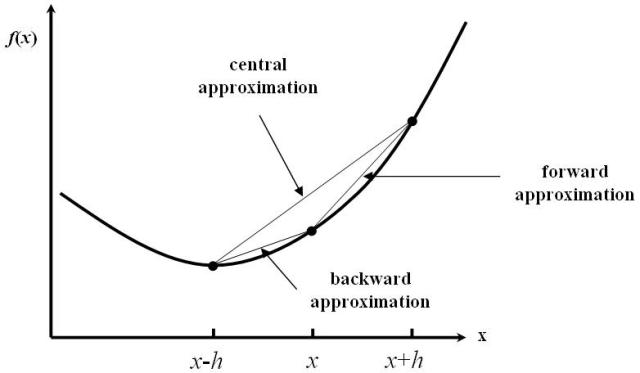
\includegraphics[width=1.0\textwidth]{images/fdiff.jpg}
\caption{First derivative approximation}
\end{figure}
\end{column}
\end{columns}
\end{frame}

\begin{frame}[label={sec:org7b20c39}]{How do these perform (accuracy) ?}
\alert{DEMO} using calculation of \(\frac{df}{dx}\)
\begin{itemize}
\item Order of accuracy depends upon the Taylor series representation (\alert{Taylor
theorem})
\item For the same function evaluations i.e. if \(n\) is the number of points
considered in our algorithm
\begin{itemize}
\item Quadrature is accurate to \(\order{h^{n+1}}\)
\item Differentation is accurate to \(\order{h^{n-1}}\)
\end{itemize}
\item Centered difference algorithms usually have a bump in order of accuracy,
for the same width of stencil
\item Lots of freedom to design own schemes\ldots{}
\end{itemize}
\end{frame}
\begin{frame}[label={sec:orgc284ca1}]{Round-off errors}
\begin{block}{Why discuss round-off errors?}
\begin{itemize}
\item Round-off errors : errors in precisely representing numbers on a computer
\item Finite precision effects were not important in quadrature, but are in
differentation.
\item \alert{Why}? Numerical differentation is susceptible to:
\begin{itemize}
\item Noise amplification
\item Cancellation errors (due to signs)
\item And as we saw last slide, is less accurate than quadrature
\end{itemize}
\end{itemize}
\end{block}
\begin{block}{Effect of round-off}
\begin{itemize}
\item If \(\epsilon\) is machine precision \(2^{-52} \approx 10^{-16}\) in
double precision we can show
\end{itemize}
\[\frac{\delta f(x)}{\delta x} = \frac{f(x+h) - f(x)}{h} \approx
	f^{\prime}(x)  + \frac{h}{2}f^{\prime\prime}(x) + \frac{\epsilon \cdot
	f}{h} + \order{h^2} \]
\end{block}
\end{frame}
\begin{frame}[label={sec:org4401cfe}]{Caution!!!}
In an ideal world, we should not be taking derivatives of functions
numerically:
\begin{itemize}
\item Differentation is \emph{unbounded}:
A function with small \(\norm{f}_{\infty}\) can have arbitrarily large \(\norm{f^{\prime}}_{\infty}\) \alert{DEMO}
\item Differentiation amplifies noise:
Smooth function with small, high-frequency wiggles (common in experiments
and under-resolved simulations) can explode \alert{DEMO}
\item Numerical differentiation : subject to cancellation and round-off errors \alert{DEMO}
\end{itemize}
\end{frame}
\begin{frame}[label={sec:org3cad256}]{Soft mechanics framework}
Many spatial differentiations. More explicitly,

\[ \spot<2>{\begin{aligned}
   m_i \cdot \frac{\partial \mathbf{v}_i}{\partial t} &= \Delta^h
   \left(\frac{\mathbf{Q}_i^T\hat{\mathbf{S}}_i\boldsymbol{\sigma}^i_{\mathcal{L}}}{e_i}\right)
   +\mathbf{F}_i,\quad i=[1,n+1]
   \end{aligned}} \]
\[ \spot<3>{\begin{aligned}\frac{\hat{\mathbf{J}}_i}{e_i} \cdot \frac{\partial
	\boldsymbol{\omega}^i_{\mathcal{L}}}{\partial t} &=
	\Delta^h\left(\frac{\hat{\boldsymbol{\mathcal{B}}}_i\hat{\boldsymbol{\kappa}}_{\mathcal{L}}^{i}}{\mathcal{E}_i^3}\right) +
	\mathcal{A}^h\left(\frac{\hat{\boldsymbol{\kappa}}_{\mathcal{L}}^i\times\hat{\boldsymbol{\mathcal{B}}}_i
	\hat{\boldsymbol{\kappa}}_{\mathcal{L}}^i}{\mathcal{E}_i^3}
	\hat{\mathcal{D}}_i\right) + \left(\mathbf{Q}_i\mathbf{t}_i\times\hat{\mathbf{S}}_i\boldsymbol{\sigma}^i_{\mathcal{L}}\right)\hat{\ell}_i\\
	&+ \mathbf{C}^i_{\mathcal{L}},\quad i=[1,n] \end{aligned}}\]
\begin{block}<3->{\(\Delta^{h}\) using finite differences}
\end{block}
\end{frame}

\begin{frame}[label={sec:org7e2a051}]{The \(\Delta^{h}\) operator}
Define the \(\Delta^{h}\) operator as:
\[\mathbf{y}_{j=1, \ldots, N+1}=\Delta^{h}\left(\mathbf{x}_{i=1, \ldots,
   N}\right)=\left\{\begin{array}{ll}{\mathbf{x}_{1}} & {\text { if } j=1}
   \\ {\mathbf{x}_{j}-\mathbf{x}_{j-1}} & {\text { if } 1<j \leq N}
   \\ {-\mathbf{x}_{N}} & {\text { if } j=N+1}\end{array}\right. \]
\end{frame}
\begin{frame}[label={sec:orgb67f935},fragile]{The \(\Delta^{h}\) operator}
 Implementation using \texttt{numpy}
\begin{minted}[,fontsize=\scriptsize]{python}
import numpy as np

# Modified trapezoidal integration
def modified_diff(t_x):
    """ Modified trapezoidal integration"""
    # Pads a 0 at the end of an array
    temp = np.pad(t_x, (0,1), 'constant', constant_values=(0,0))
    # Using roll calculate the diff (ghost node of 0)
    return (temp - np.roll(temp, 1))

# data
a = np.tile(np.arange(5,), 10)
b = modified_diff(a)
\end{minted}
\end{frame}
\begin{frame}[label={sec:orgdb31dc0}]{Credits}
\begin{block}{A good chunk of the material in these slides are taken from Prof. Andreas Kloeckner's CS450 lectures and Prof. Paul Fischer's TAM470 lectures}
\end{block}
\end{frame}
\end{document}
